\chapter{Généralités sur les drones}
% \addstarredchapter{Introduction} %Sinon cela n'apparait pas dans la table des matières
% \markboth{Introduction}{Introduction} % headers

% \chapter{}
% \minitoc
% \newacronym{gcd}{GCD}{Greatest Common Divisor}
% \todo{contexte}

% \section{Drones autonomes}
Ces dernières années, le domaine des drones s'est considérablement développé. En effet, de nombreux progrès ont été réalisés dans la conduite de vols autonomes, lesquels permettent de réaliser de nombreuses taches longues, répétitives ou dangereuses, de manière plus sûre que des avions ou des systèmes télépilotés. Les drones ont fait leurs preuves dans de nombreuses applications civiles, alors qu'ils étaient auparavant conçus à des fins de surveillance et de destruction dans le secteur militaire.

La possibilité d'utiliser des systèmes de vols autonomes dans le secteur civil a été rendu possible par l'accessibilité croissante, proposée par l'industrie, de solutions à faible coût pour les applications d'imagerie aérienne. Ainsi, ce sont dans des domaines aussi variés que l'agriculture de précision,  l'inspection des infrastructures civiles ou encore les opérations de sécurité que les drones autonomes sont aujourd'hui mobilisés, devenant alors un riche sujet de recherche.

La miniaturisation des équipements électroniques et mécaniques est à l'origine de l'essor d'une classe de drones de plus en plus petits. Souvent qualifiés de \textit{Micro Air Vehicle} (MAV), leur petite taille leur permet d'intervenir dans des espaces confinés ou contraints. Ils n'ont, cependant, qu'une charge utile restreinte, souvent limitée à l'emport d'une caméra ou d'un colis de faible masse. 
\nomenclature[]{\(MAV\)}{Micro drone (\textit{Micro Air Vehicle})}
Leur faible autonomie restreignant leur usage, la recherche s'est alors concentrée sur une solution permettant d'optimiser leur utilisation. En cela, les drones à décollage et atterrissage vertical (\textit{Vertical take-off and landing}; VTOL) répondent aux exigences.
\nomenclature[]{\(VTOL\)}{Drones à décollage et atterrissage vertical (\textit{Vertical take-off and landing})}

\section{Micros drones convertibles}

    \subsection{Domaine de vol} 
    Tout l'intérêt d'un drone convertible réside dans sa capacité à décoller et atterrir verticalement, tout en conservant une bonne efficacité énergétique en vol d'avancement, grâce par une aile. Cette aile a l'avantage de générer de la portance, laquelle s'oppose au poids du drone et permet d'assurer sa sustentation. La contrepartie de la génération de la portance est la traînée qui s'oppose à l'avancement et doit être contrée par une force de traction générée par les hélices. Nous pouvons définir l'efficacité énergétique comme le ratio entre le temps de vol et l'énergie électrique nécessaire pour effectuer ce vol.
    
    Afin de souligner la prééminence de l'efficacité énergétique de ce modèle convertible, il convient de la comparer avec celle d'un drone quadrirotor qui assure sa sustentation uniquement grâce à des hélices (à l'instar d'un hélicoptère), et à celle d'un drone à voilure fixe.
    \todo{Completer}
    \begin{table}[ht]
        \centering
        \begin{tabular}{|c|c|c|c|c|}
            \hline
            Architecture & Vitesse $\SI{}{\meter\per\second}$  & Stationnaire & Temps de vol & Consommation\\
            \hline \hline
            Convertible & [0 - 30] & Possible & Quelques heures & Faible\\
            \hline
            Quadrirotor & [0 - 16] & Possible& Quelques minutes & Forte\\
            \hline
            Voilure fixe & [8 - 30] & Impossible & Plusieurs heures & Variable \\
            \hline
        \end{tabular}
        \caption{Comparaison des architectures de drone.}
    \end{table}
    % Drone à voilure fixe, stationnaire impossible, grande efficité ernegetique vitesse mini et max
    % Quadrirotor, grande manouvrabilité, faible efficaité energetique
    % Convertible, dommaine de vol important, sensibilité aux pertubation, grand efficaticté energetique en vol d'avancement, faible en stationnaire 

    Nous observons qu'un drone convertible possède un domaine de vol bien plus important qu'un drone à voilure fixe, lequel ne sera pas en mesure de voler à très basse vitesse et qu'un quadrirotor, dont l'autonomie va être limitée par sa consommation.
    En alliant autonomie et vol stationnaire, le modèle convertible répond aux exigences des missions civiles et militaires.

    \subsection{Types d'architecture des drones convertibles}
    La conception structurelle et aérodynamique d'un drone est le facteur principal permettant des transitions stables et fluides. De plus, il est nécessaire d'optimiser l'architecture pour une mission, de manière à être le plus efficace. Au vu de la diversité des tâches à réaliser, un grand nombre de modèles ont été proposés, lesquels sont catégorisables en quatre classes : \textit{quadplanes}, \textit{tiltrotor}, \textit{tailsitter}, \textit{tiltwing}. 
    En ce qu'il s'agit des prémices des convertibles, il parait opportun d'ajouter aux trois grandes catégories classiquement citées dans les états de l'art (\textit{tiltrotor}, \textit{tailsitter}, \textit{tiltwing}) \cite{saeed_survey_2018,ducard_review_2021, review_2022}, la catégorie \textit{quadplanes}.

        \subsubsection*{\textit{Quadplanes}}
        Les \textit{quadplanes} résultent de la fusion d'un avion et d'un quadrirotor (comme visible sur la figure \ref{fig:quadplane}), ce qui permet un découplage de l'actionnement en fonction de la phase de vol. Le premier système de propulsion est composé de quatre hélices générant une force verticale permettant le contrôle lors de phase de décollage, d'atterrissage et stationnaire. Le second système de propulsion est composé d'une hélice propulsive supplémentaire afin de maintenir le vol d'avancement.

        \begin{figure}[ht]
            \centering
                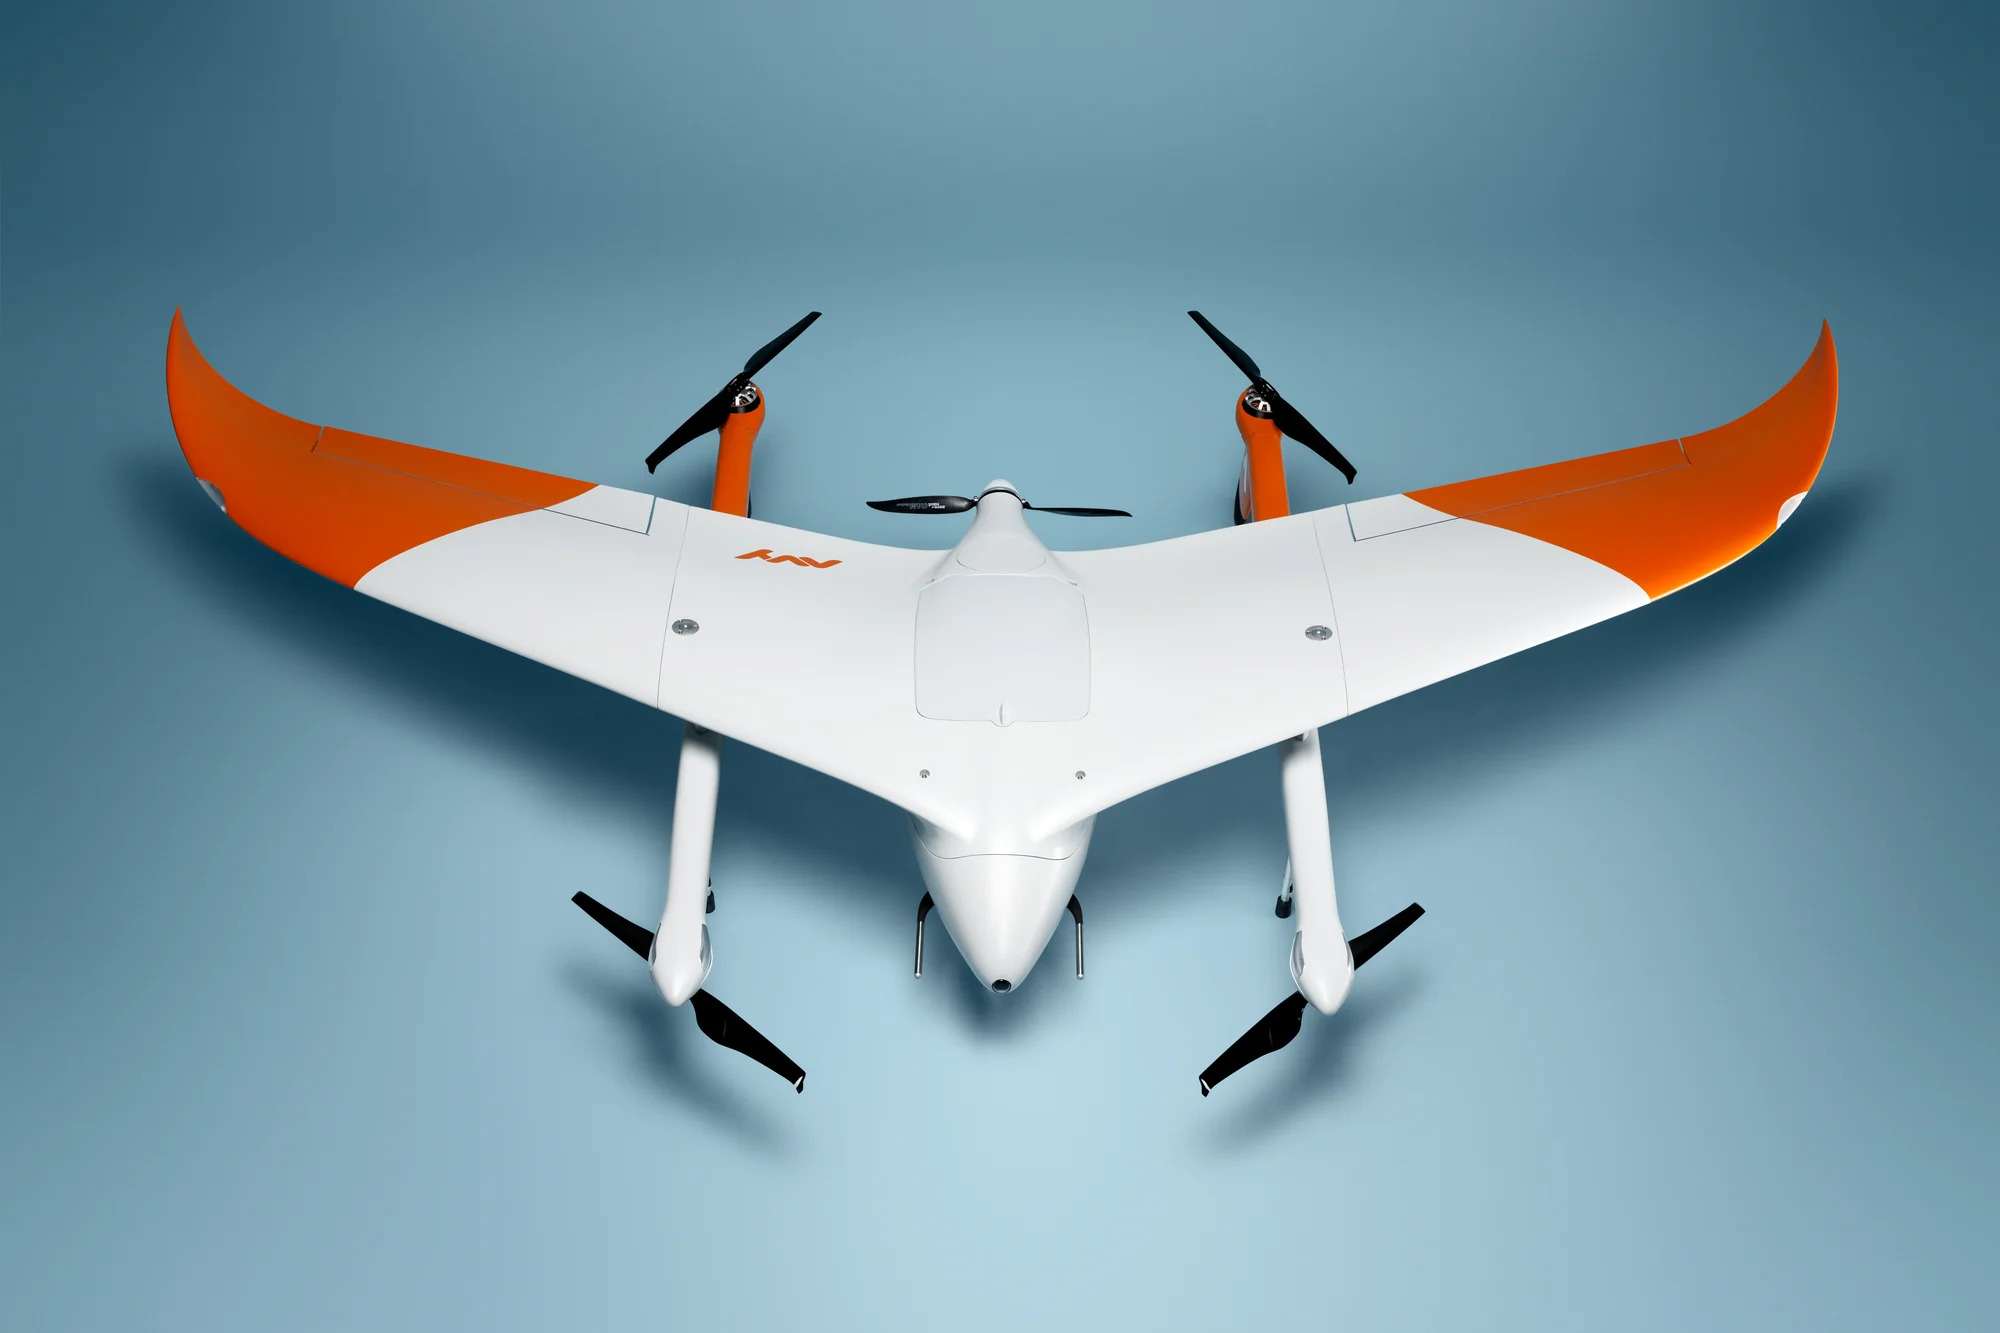
\includegraphics[width=0.6\columnwidth]{figures/Avy-Drone-quadplane.jpg}
                \caption{Structure \textit{quadplanes} proposée par \cite{Avy_2023}.}
                \label{fig:quadplane}
        \end{figure}
        

        L'avantage de ce type d'architecture est sa grande robustesse. Effectivement, aucune pièce en mouvement n'est nécessaire pour réaliser la transition, ce que réduit le risque de défaillance mécanique. Toutefois, l'inconvénient réside dans son manque d'efficacité. Lors d'un vol d'avancement, la portance sera générée par l'aile. Ainsi, il est possible de désactiver les rotors qui génèrent des perturbations aérodynamiques et des trainées parasites. Les axes des moteurs se retrouvent orthogonaux au flux d'air généré par le déplacement du drone, ce qui correspond au cas le plus défavorable en termes de trainée. De plus, la surcharge engendrée par l'emport de moteurs supplémentaires se traduit par une diminution de la charge utile transportable. 

        En termes de contrôle, un atout indéniable est la séparation des actionnements en fonction des phases de vols. Ainsi, l'architecture de commande sera basée sur un mécanisme de commutation permettant de choisir la loi de commande appropriée sur un critère de vitesse air. Ce critère est pertinent en ce qu'il est lié à la capacité de l'aile à générer de la portance induite par le flux d'air. Ainsi, à basse vitesse, le drone se stabilise avec l'actionnement quadrirotor et la loi de commande associée. Dans les vitesses plus importantes, la commutation de la loi permet de contrôler le drone en mode avion. Toutefois, le passage d'une loi à l'autre reste le point clé de la commande et demeure complexe et critique.

        \subsubsection*{\textit{Tiltrotor}}

        Les \textit{tiltrotor} nécessitent l'utilisation d'un actionneur dédié à la modification de l'orientation des moteurs. Les rotors sont montés sur des arbres basculants actionnés et la transition du vol stationnaire au vol d'avancement (ou inversement) s'effectue progressivement en fonction de l'inclinaison du rotor. {\color{blue}Les deux configurations sont représentés sur la figure \ref{fig:tiltrotor}.} Ainsi, l'angle entre le souffle des hélices et l'aile peut être ajusté à chaque instant. Cet angle joue un rôle important dans le contrôle des forces et des moments aérodynamiques : sa maîtrise permet de mieux gérer, non seulement, les performances aérodynamiques du vol lors des transitions, mais aussi la stabilité du système sur l'ensemble du domaine de vol. 
        Malgré le fait que les \textit{tiltrotor} embarquent un actionneur uniquement dédié à la transition, ce qui augmente la masse du drone, cette architecture est intéressante car elle permet d'utiliser les mêmes actionneurs pour assurer la sustentation en stationnaire et pour générer la traction en mode avion.
        \begin{figure}[ht]
            \centering
            \resizebox{.9\textwidth}{!}{%
            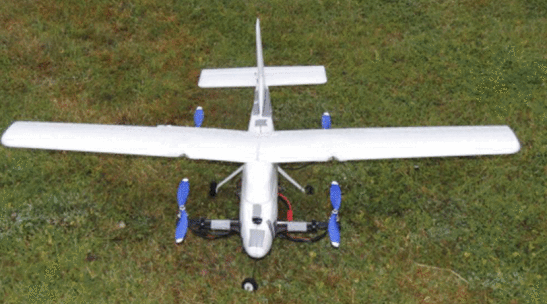
\includegraphics[height=3cm]{figures/tiltrotorhover.png}
            \quad
            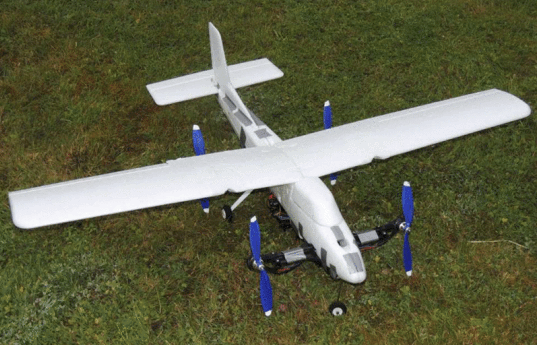
\includegraphics[height=3cm]{figures/tiltrotorforward.png}
            }
            \caption{Structure \textit{Tiltrotor}  proposée par \cite{7040348}, dans deux configurations, vol stationnaire et d'avancement.}
            \label{fig:tiltrotor}
        \end{figure}


        

        \subsubsection*{\textit{Tailsitter}}
        Contrairement au \textit{tiltrotor} qui se pose sur le fuselage de l'avion (figure \ref{fig:tiltrotor}), les \textit{tailsitter} se posent à la verticale (voir figure centrale \ref{fig:tailsitter}). Durant la transition du mode stationnaire au vol d'avancement, la structure entière bascule vers l'avant modifiant l'angle d'incidence de la voiture. Selon la configuration du \textit{tailsitter}, la transition peut être réalisée soit par la génération du moment aérodynamique créé par les élevons, soit par le couple créé par le système de propulsion. Pendant le vol d'avancement, en position horizontale, le \textit{tailsitter} vole comme un avion conventionnel sans dérive. En utilisant des techniques aérodynamiques classiques, les concepteurs peuvent optimiser le profil de l'aile du \textit{tailsitter} pour le rendre plus endurant afin de réduire la consommation d'énergie. Grâce à ce processus d'optimisation aérodynamique, le \textit{tailsitter} peut effectuer des missions de vol de plus d'une heure.

        \begin{figure}[ht]
            \centering
            \resizebox{.9\textwidth}{!}{%
            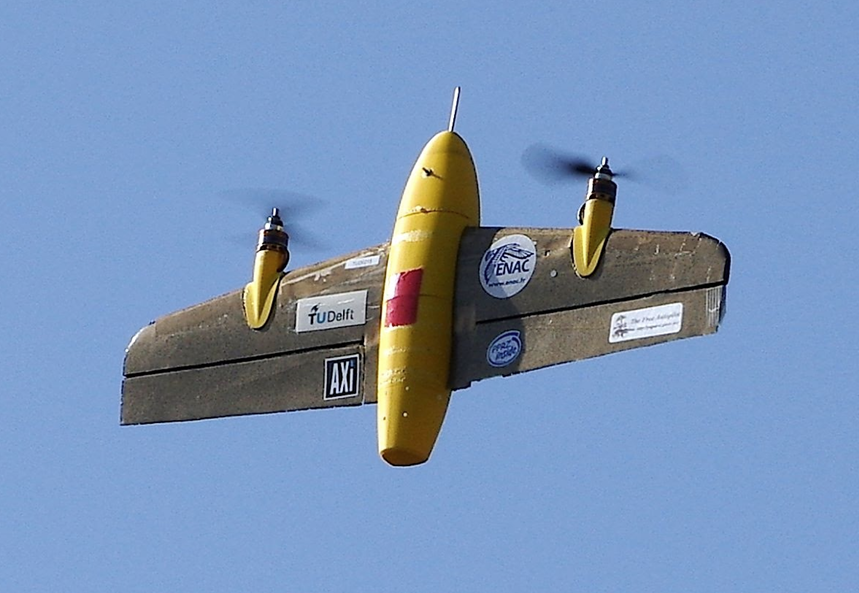
\includegraphics[height=3cm]{figures/cyclone.png}
            \quad
            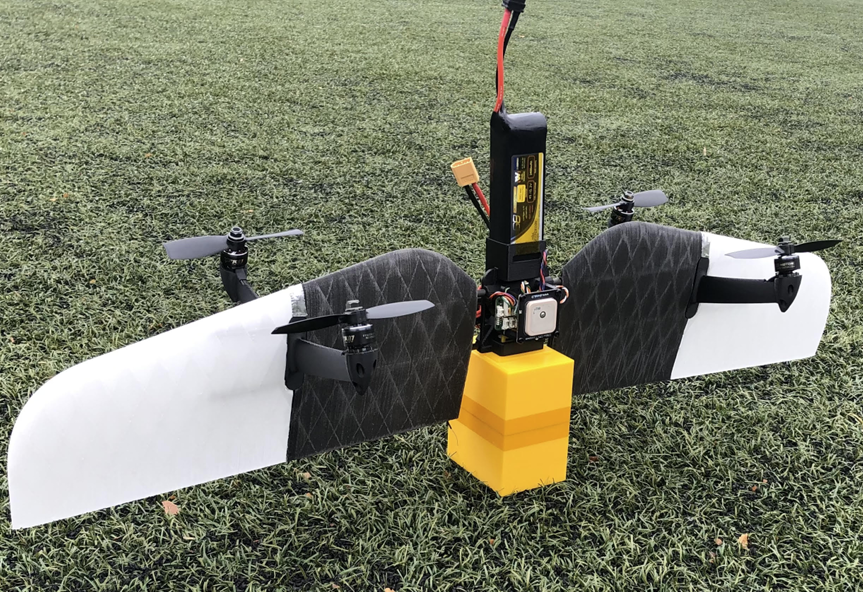
\includegraphics[height=3cm]{figures/falcon.png}
            \quad
            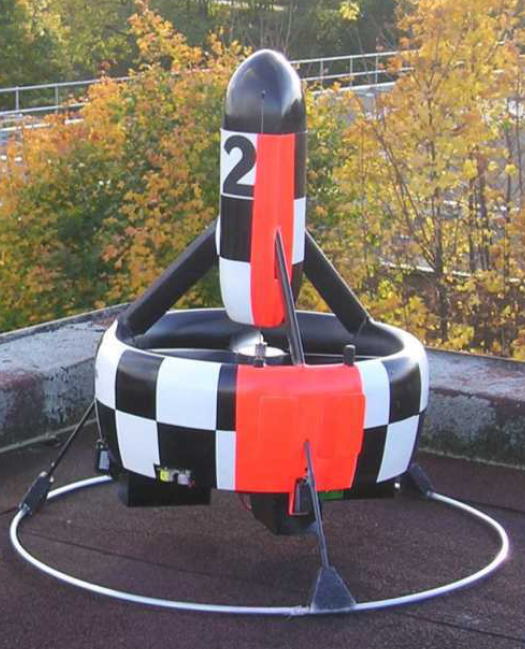
\includegraphics[height=3cm]{figures/HoverEye.png}
            }
            \caption{Structure \textit{tiltrotor}  proposée par \cite{Smeur_2020,fernandez:hal-04612206,pflimlin:tel-00132352}.}
            \label{fig:tailsitter}
        \end{figure}
        
        Ce modèle semble être la configuration la plus aboutie des drones convertibles, car il utilise les mêmes actionneurs dans tout le domaine de vols. Ainsi, aucune masse superflue n'est embarquée.

    
        \subsubsection*{\textit{Tiltwing}} 
        La particularité des \textit{tiltwings} réside dans le fait que les rotors sont inclinés en même temps que les ailes (voir figure \ref{fig:tiltwing}). Un actionneur supplémentaire et puissant est donc nécessaire pour surmonter le couple de l'aile afin de la positionner dans l'orientation souhaitée. La commande de cet actionneur doit être prise en compte lors de la conception des lois de commande. Pendant le décollage, l'atterrissage et les vols stationnaires, les ailes doivent être positionnées vers le haut afin de produire une force de poussée opposée au vecteur gravité. Dans ces phases de vol, lorsque les ailes sont orientées vers le haut, l'aéronef est plus vulnérable aux vents et les lois de commande doivent rejeter ces perturbations. Dans la littérature, il existe plusieurs configurations d'ailes basculantes et différentes approches de contrôle conçues pour stabiliser leur dynamique de vol.
        % \cite{}.
        \todo{cite}
        \begin{figure}[ht]
            \centering
            \resizebox{.9\textwidth}{!}{%
            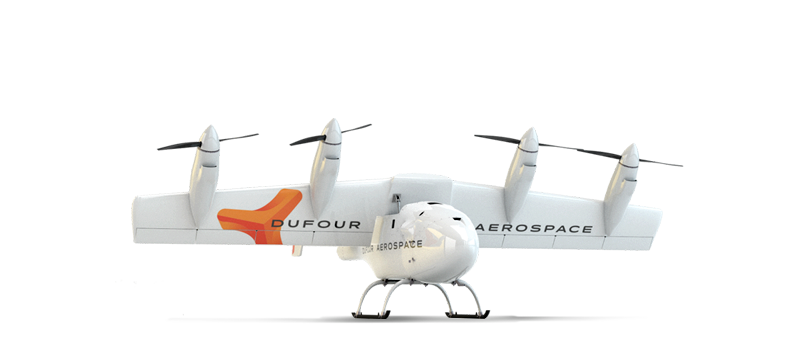
\includegraphics[height=3cm]{figures/tiltwing_aero2.png}
            \quad
            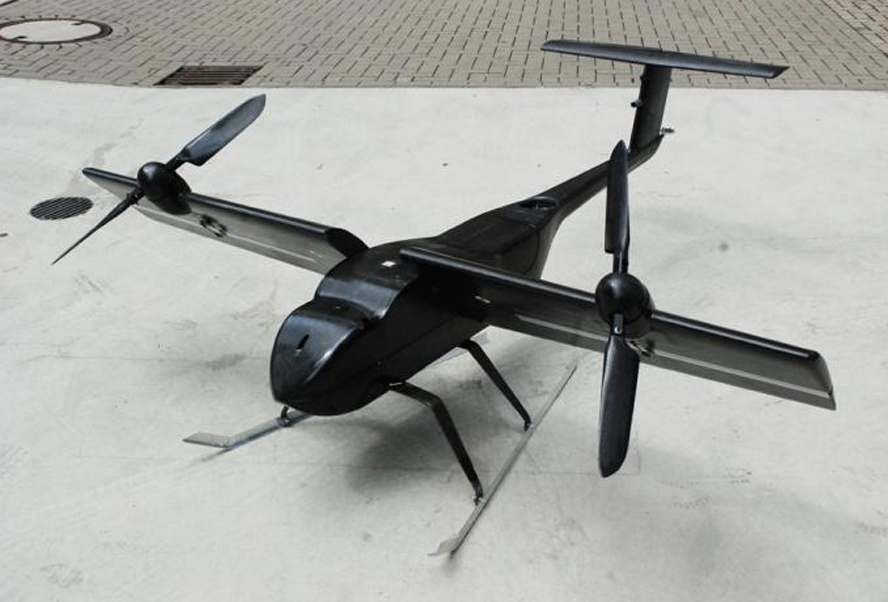
\includegraphics[height=3cm]{figures/avigle_tiltwing.png}
            }
            \caption{Structure \textit{tiltwings}  proposée par \cite{Aero2_2024, Ostermann2012ControlCO}.}
            \label{fig:tiltwing}
        \end{figure}

        Par ailleurs, les \textit{freewing} sont une gamme en cours de développement à l'intérieur de l'architecture des \textit{tiltwing}. Ils sont actionnés comme des \textit{tiltwing} sauf au niveau de l'axe de rotation entre l'aile et le fuselage. Cette rotation est laissée libre, ce degré de liberté permet à l'aile de changer librement son incidence. {\color{blue} Il résulte un gain de masse car il est possible de se supprimer de l'actionneur puissant et lourd nécessaire à la rotation de l'aile. De plus, l'aile étant libre de s'orientée, les turbulences ont un impact plus faible sur la structure, ce qui rends les vols plus stables \cite{freewing2012, Johnson2021, Johnson2023}. }


\section{Propriétés des \textit{tailsitters} et des \textit{freewings}}
    D'un point de vue mécanique, les \textit{tailsitters} et les \textit{freewings} sont caractérisés comme des systèmes sous-actionnés avec une dynamique fortement couplée. Ces caractéristiques mécaniques rendent le processus de modélisation et d'identification difficile. Cela peut s'expliquer par le fait que, pour ce type de système, une entrée de commande donnée agit simultanément sur différentes dynamiques. Ainsi, l'identification de l'influence d'une entrée de commande donnée sur une dynamique particulière reste un processus important qui nécessite plus d'attention.
    \subsection{Actionnement}
    Dans ces deux architectures, il est courant de trouver des actionneurs basés sur des effets aérodynamiques. Ces actionneurs ont l'avantage d'être peu consommateur en énergie. Ils sont mus par des servomoteurs qui consomment peu d'électricité proportionnellement au couple qu'ils génèrent. Dans le cas des ailes volantes, les surfaces aérodynamiques sont souvent placées sur la partie arrière des ailes et peuvent être utilisées symétriquement à l'instar de volets ou anti-symétriquement comme des ailerons. 
    Dans les phases de vol stationnaire, d'atterrissage ou de décollage, la plateforme est maintenue en vol par les hélices ; ainsi, il est nécessaire de dimensionner les groupes moteurs-hélices pour qu'ils puissent générer assez de force. En fonction des configurations, les moments peuvent être obtenus par des différentiels sur l'utilisation des moteurs ou bien par des surfaces aérodynamiques. Dans le cas de surfaces soufflées par le flux d'air des hélices, il existe un couplage des actionneurs qui complexifie la modélisation et le contrôle de ces architectures.

    \subsection{Aérodynamique}

    Lors d'un vol d'avancement ces architectures assure le maintien du vol en palier en générant une force de portance grâce à leurs surfaces alaires. Cette portance s'oppose au poids permettant de suivre une trajectoire. La force de trainé engendré par l'aile et le fuselage et compensé par la composante horizontale de la poussée. En vol stationnaire, le poids est compensé par la traction de l'hélice. La relation d'équilibre est plus complexe lorsque nous évaluons l'ensemble des points d'équilibre de la transition d'un mode à l'autre. La transition équilibrée est assurée par le mélange correct des forces aérodynamiques et de propulsion.

    Les interactions aérodynamiques entre l'hélice et la surface de l'aile sont connues pour être complexe et difficile à modéliser. La vitesse induite par le souffle de l'hélice entraîne une variation locale de l'angle d'attaque et des variations de pression dynamique au niveau des sections d'aile immergées, d'où une distribution différente de la portance. L'analyse de l'interaction entre l'hélice, l'aile et les élevons doit permettre d'obtenir de bonnes caractéristiques de vol et de tirer profit des combinaisons. C'est pour cela que l'on trouve dans la littérature différents travaux de recherche sur l'interaction hélice-aile 
    % \cite[text]{keylist}.
     L'identification de ces effets aérodynamiques nécessite, pour chaque point de vol, les informations de l'air environnant, les valeurs des entrées de commande et les mesures des forces et moments aérodynamiques agissant sur le système. Le moyen le plus précis et le plus fiable d'identifier les phénomènes aérodynamiques est probablement de mener des campagnes en soufflerie, qui sont coûteuses et prennent beaucoup de temps.


\section{Modélisations}
Dans le cas des drones convertible basculant, le modèle aérodynamique doit être valide dans les phases de transition. Cela nécessite l'extension de l'aérodynamique classique (faible incidence) à un angle d'attaque élevé et à un fonctionnement à faible vitesse. En outre, l'effet du souffle de l'hélice sur les profils aérodynamiques du véhicule doit être compris et pris en compte dans le modèle du système. Par exemple, les travaux de \cite{9444145} sur un \textit{tiltwing}, identifient les zones d'interaction entre l'hélice et l'aile. Ils séparent clairement la génération de force et de couple induite par l'aile soufflé et non-soufflé.

Des fonctions non linéaires continues décrivant les coefficients de portance et de traînée aérodynamiques sur toute la plage de l'angle d'attaque pour les  \textit{tiltrotors} ont été dérivées dans \cite{6981467} et pour les \textit{tiltwing} dans \cite{lustosaHal-03035938,Lustosa2017LaP}.

Il existe de nombreuses conceptions possibles pour un drone convertible. Bien que tous les modèles aient une structure commune, il existe des différences majeures dans la formulation réelle des termes de force et de couple. Celles-ci dépendent de la disposition des moteurs ou des hélices, de l'existence ou non de surfaces de contrôle aérodynamiques et de la forme du véhicule.

Un modèle de véhicule précis est nécessaire pour les conceptions classiques de contrôle basées sur un modèle et en particulier pour les approches d'inversion dynamique ou de contrôle prédictif de modèle. Cependant, un modèle précis va nécessite du travail pour être pertinent. La précision va être obtenu à l'aide de campagne d'identification longue et complexe en soufflerie ou à l'aide de vol en environnement contraint. Il se peut aussi que le modèle soit complexe au point de ne pas pouvoir l'utiliser directement dans le contrôle à cause de limitation matérielle des calculateurs embarqué.


Dans notre cas, nous nous sommes intéressé à l'impact du vent sur les architectures mentionné précédent. Il est donc nécessaire de modéliser le vent. Dans le cas de vent constant ou de cisaillement de vent un modèle à échelon semble tout à fait approprié pour représenter le changement brusque de vitesse de vent. 
Pour les rafales, nous utiliserons plusieurs modèles. Nous pouvons utiliser le modèle "Chapeau mexicain" ou les "ondelette de Morlet".

La fonction définissant le chapeau mexicain est :
\begin{align}
    \Psi_{mex}(t)= w_{m} - \frac{A_g}{2} \left(1-\cos(2 \pi f_g (t-t_{0,mex}))\right)\sin(3 \pi f_g (t-{0,mex}))
\end{align}
et la fonction ondelette de Morlet est défini par :
\begin{align}
    \Psi_{mor}(t)=  w_{m} + A_g \exp(-(t+t_{0,mor})) \cos(5*(t-t_{0,mor}))
\end{align}
où $w_{m}$ est le vent moyen sans perturbation, $t_{0,mex}$ représente l'instant de début de perturbation et $t_{0,mor}$ l'instant où la perturbation est maximale, $A_g$ est l'intensité maximale de la perturbation et  $f_g$ est la fréquence de la perturbation. Les tracées de la figure \ref{fig:mexhat} montre la représentation temporelle des deux fonctions pour les valeurs $w_{m} = \SI{1}{\meter\per\second}$, $t_{0,mex} = \SI{2}{\second}$,  $t_{0,mor} = \SI{5}{\second}$, $A_g = \SI{1}{\meter\per\second}$ et $f_g = \SI{0.8}{\radian\per\second}$.


\begin{figure}[ht!]
    \centerline{
    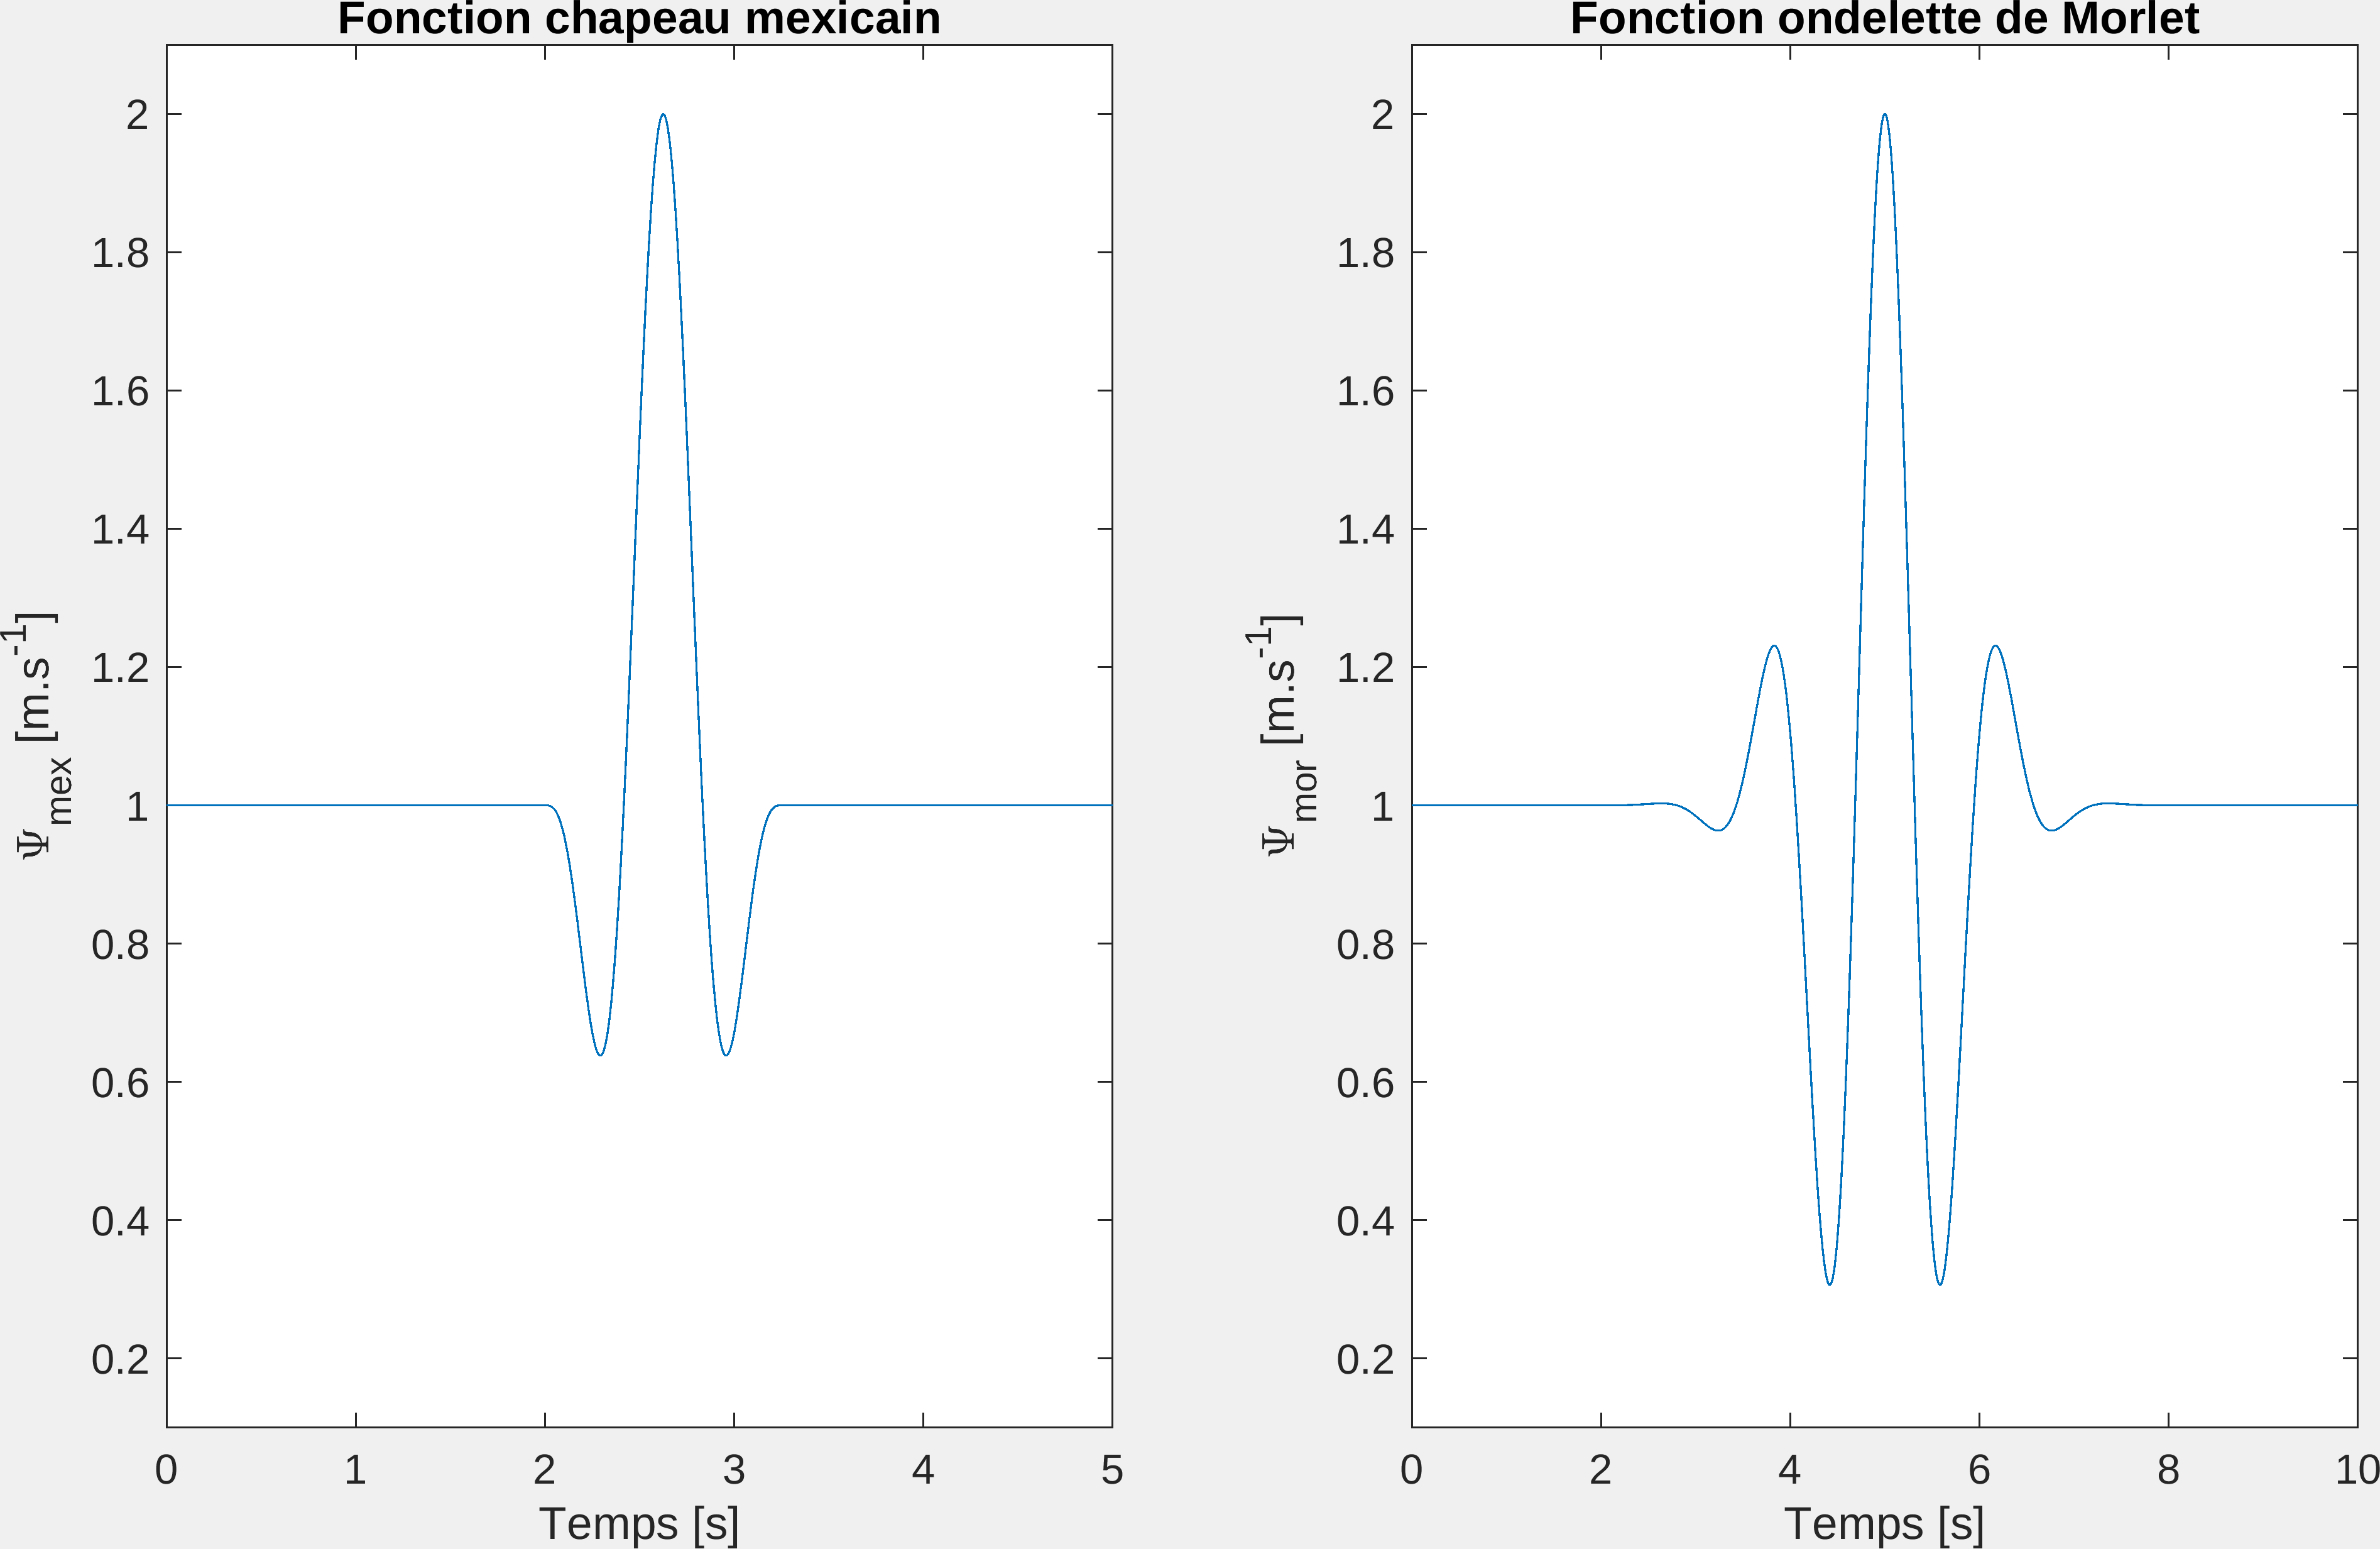
\includegraphics[trim=0cm 0cm 0cm 0cm,clip,width=0.8\columnwidth]{figures/mex_hat_morlet.png}}
    \caption{Représentation temporelle des modèles de perturbations de vent.}
    \label{fig:mexhat}
\end{figure}

Le modèle de Dryden est defini
\begin{subequations}
    \begin{align}
        \Phi _{u_{g}}(\Omega )& =\sigma _{u}^{2}{\frac {2L_{u}}{\pi }}{\frac {1}{1+(L_{u}\Omega )^{2}}}\\
        \Phi _{v_{g}}(\Omega )& =\sigma _{v}^{2}{\frac {2L_{v}}{\pi }}{\frac {1+12(L_{v}\Omega )^{2}}{\left(1+4(L_{v}\Omega )^{2}\right)^{2}}}\\
        \Phi _{w_{g}}(\Omega )& =\sigma _{w}^{2}{\frac {2L_{w}}{\pi }}{\frac {1+12(L_{w}\Omega )^{2}}{\left(1+4(L_{w}\Omega )^{2}\right)^{2}}}
    \end{align}
\end{subequations}

Le modèle de von Kármán
\begin{subequations}
    \begin{align}
        \Phi _{u_{g}}(\Omega )& =\sigma _{u}^{2}{\frac {2L_{u}}{\pi }}{\frac {1}{\left(1+(1.339L_{u}\Omega )^{2}\right)^{\frac {5}{6}}}}\\
        \Phi _{v_{g}}(\Omega )& =\sigma _{v}^{2}{\frac {2L_{v}}{\pi }}{\frac {1+{\frac {8}{3}}(2.678L_{v}\Omega )^{2}}{\left(1+(2.678L_{v}\Omega )^{2}\right)^{\frac {11}{6}}}}\\
        \Phi _{w_{g}}(\Omega )& =\sigma _{w}^{2}{\frac {2L_{w}}{\pi }}{\frac {1+{\frac {8}{3}}(2.678L_{w}\Omega )^{2}}{\left(1+(2.678L_{w}\Omega )^{2}\right)^{\frac {11}{6}}}}
    \end{align}
\end{subequations}


\section{Commandes}

\begin{figure}[ht!]
    \centerline{
    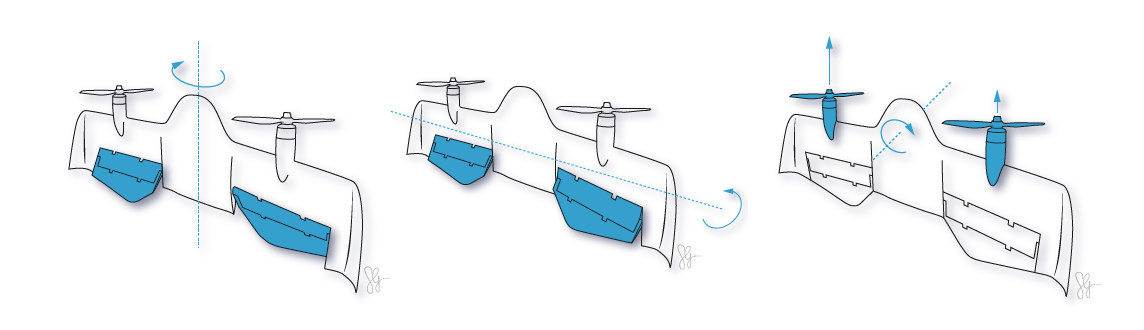
\includegraphics[trim=0cm 0cm 0cm 0cm,clip,width=0.8\columnwidth]{figures/imageActionnementDarko.png}}
    \caption{Todo.}
    \label{fig:actionDarko}
\end{figure}
\todo{add axes on picture}

La figure \ref{fig:actionDarko} illustre les effets des actionneurs sur la dynamique de l'attitude des \textit{tailsitters}. L'angle de roulis  peut être contrôlé par des braquages de volets asymétriques, l'angle de tangage par des braquages de volets symétriques et la rotation autour de l'axe de lacet est contrôlée par un dispositif de poussée différentielle, ce qui permet d'obtenir un angle de tangage plus élevé. La rotation autour de l'axe de lacet est contrôlée par une configuration de poussée différentielle, qui crée un couple temporaire non nul autour de son axe. Le dispositif de poussée différentielle crée une différence entre les rotations de l'hélice gauche et de l'hélice droite, et modifie ainsi la vitesse de rotation de l'avion et modifie ainsi le comportement aérodynamique autour des volets.

\section{Présentation de la thèse}
L'étude des drones convertibles est un point central de notre travail. Nous nous intéresserons à deux architectures, dans un premier temps un \textit{tailsitters}, DarkO puis dans un second temps un \textit{freewings}, Colibri, basée sur une aile inspiré de DarkO en rotation libre autour d'un fuselage qui sera maintenu horizontal.

